%
% This work is licensed under a Creative Commons Attribution-ShareAlike 4.0 International License.
% http://creativecommons.org/licenses/by-sa/4.0/
%

% DO NOT COMPILE THIS FILE DIRECTLY!
% This is included by the other .tex files.


\begin{frame}
    
\includegraphics[scale=0.3]{images/logo-circl-Forensics.png}
    \begin{itemize}
        \item[]
        \item[]
        \item[] 6. Forensics Challenges
    \end{itemize}
\end{frame}


\begin{frame}[fragile]
  \frametitle{6.1 Hide and recover data}
  \begin{itemize}
    \item Situation:
    \begin{itemize}
      \item USB stick image
      \item One partition
      \item Several unallocated sectors
      \item[]
    \end{itemize}
    \item Challenge:
    \begin{itemize}
      \item Hide a message in unallocated sector
      \item Recover the message
      \item Hide a binary in unallocated sectors
      \item Recover the binary
      \item[]
    \end{itemize}
  \end{itemize}
\end{frame}


\begin{frame}[fragile]
  \frametitle{6.1 Hide and recover data}
  \begin{lstlisting}[basicstyle=\tiny]
1. Hide message in the last (unallocated) sector
------------------------------------------------
    echo -n "My secret message" | dd of=mbr_ex.raw seek=262143 status=none conv=notrunc


2. Read message from the last (unallocated) sector
--------------------------------------------------
    dd if=mbr_ex.raw skip=262143 status=none | xxd | less
    dd if=mbr_ex.raw skip=262143 status=none | strings


3. Hide a binary file between MBR and 1th partition
---------------------------------------------------
    dd if=/bin/dd of=mbr_ex.raw seek=3 conv=notrunc
        76000 bytes (76 kB, 74 KiB) copied, 0,00173009 s, 43,9 MB/s


4. Recover the hidden binary file
---------------------------------
    dd if=mbr_ex.raw skip=0 count=4 | xxd | less

    dd if=mbr_ex.raw bs=1 skip=$((3*512)) count=76000 of=ddddd.exe
        76000 bytes (76 kB, 74 KiB) copied, 0,12853 s, 591 kB/s

    md5sum ddddd.exe /bin/dd 
        36a70f825b8b71a3d9ba3ac9c5800683  ddddd.exe
        36a70f825b8b71a3d9ba3ac9c5800683  /bin/dd
  \end{lstlisting}
\end{frame}


\begin{frame}[fragile]
  \frametitle{6.2 Recovering corrupt MBR}
  \begin{itemize}
    \item Situation:
    \begin{itemize}
      \item USB stick image
      \item Several partitions available
      \item At least one partition do not mount
      \item[]
    \end{itemize}
    \item Challenge:
    \begin{itemize}
      \item Examine the partition table
      \item Find the first sector of the partition
      \item Fix the Master Boot Record - MBR
      \item Analyze the other offsets
      \item Analyze unallocated sectors
      \item[]
    \end{itemize}
  \end{itemize}
\end{frame}


\begin{frame}[fragile]
  \frametitle{6.2 Recovering corrupt MBR}
  \begin{lstlisting}[basicstyle=\tiny]
1. Examine the partition table
------------------------------
    $ fdisk -l mbr/mbr_ex.raw 
        Sector size (logical/physical): 512 bytes / 512 bytes
        Disklabel type: dos
        Disk identifier: 0x9392806f

        Device          Boot  Start    End Sectors Size Id Type
        mbr/mbr_ex.raw1        2050  67585   65536  32M  c W95 FAT32 (LBA)
        mbr/mbr_ex.raw2       67586 133119   65534  32M  c W95 FAT32 (LBA)
        mbr/mbr_ex.raw3      133120 262142  129023  63M  c W95 FAT32 (LBA)
  
  
    $ mmls mbr/mbr_ex.raw
        DOS Partition Table
        Offset Sector: 0
        Units are in 512-byte sectors

              Slot      Start        End          Length       Description
        000:  Meta      0000000000   0000000000   0000000001   Primary Table (#0)
        001:  -------   0000000000   0000002049   0000002050   Unallocated
        002:  000:000   0000002050   0000067585   0000065536   Win95 FAT32 (0x0c)
        003:  000:001   0000067586   0000133119   0000065534   Win95 FAT32 (0x0c)
        004:  000:002   0000133120   0000262142   0000129023   Win95 FAT32 (0x0c)
        005:  -------   0000262143   0000262143   0000000001   Unallocated
  \end{lstlisting}
\end{frame}


\begin{frame}[fragile]
  \frametitle{6.2 Recovering corrupt MBR}
  \begin{lstlisting}[basicstyle=\tiny]
2. Investigate start of 1th partition
-------------------------------------
    dd if=mbr/mbr_ex.raw skip=2050 count=1 status=none | xxd | less
    dd if=mbr/mbr_ex.raw skip=2047 count=4 status=none | xxd | less


Fix LBA Start vaule of 1th partition entry
------------------------------------------
    Calculation: 2048 = 0x00000800 => little endian: 0X00080000
        Replace 0X02080000 with 0X00080000

    hexedit -l 16 mbr/mbr_ex.raw
        000001C0   21000C34  30040008  00000000  01000033


Review partition table and file system stats
--------------------------------------------
    mmls mbr/mbr_ex.raw 
              Slot      Start        End          Length       Description
        000:  Meta      0000000000   0000000000   0000000001   Primary Table (#0)
        001:  -------   0000000000   0000002047   0000002048   Unallocated
        002:  000:000   0000002048   0000067583   0000065536   Win95 FAT32 (0x0c)
        003:  -------   0000067584   0000067585   0000000002   Unallocated
        004:  000:001   0000067586   0000133119   0000065534   Win95 FAT32 (0x0c)
        005:  000:002   0000133120   0000262142   0000129023   Win95 FAT32 (0x0c)
        006:  -------   0000262143   0000262143   0000000001   Unallocated
  \end{lstlisting}
\end{frame}


\begin{frame}[fragile]
  \frametitle{6.2 Recovering corrupt MBR}
  \begin{lstlisting}[basicstyle=\tiny]
3. Investigate end of 1th and start of 2nd partition
----------------------------------------------------
    fsstat -o 2048 mbr/mbr_ex.raw
        File System Type: FAT16
        Total Range: 0 - 65535
	....
	--> Size of partition 1 is okay


    sigfind -o 510 -l AA55 mbr/mbr_ex.raw
        Block: 0 (-)
        Block: 2048 (+2048)
        Block: 67586 (+65538)
        Block: 133120 (+65534)


    fsstat -o 67586 mbr/mbr_ex.raw
        File System Type: FAT16
        Total Range: 0 - 65533
        ....
	--> Start of partition 2 is okay
	--> There are 2 unallocated sectors in between
	--> Size of partition 2 is okay 


Investigate the sectors
-----------------------
    dd if=mbr/mbr_ex.raw skip=67583 count=4 | xxd | less
  \end{lstlisting}
\end{frame}


\begin{frame}[fragile]
  \frametitle{6.2 Recovering corrupt MBR}
  \begin{lstlisting}[basicstyle=\tiny]
        005:  000:002   0000133120   0000262142   0000129023   Win95 FAT32 (0x0c)
        006:  -------   0000262143   0000262143   0000000001   Unallocated

  
4. Investigate 3rd partition
----------------------------
    sigfind -o 510 -l AA55 mbr/mbr_ex.raw
        Block: 0 (-)
        Block: 2048 (+2048)
        Block: 67586 (+65538)
        Block: 133120 (+65534)


    fsstat -o 133120 mbr/mbr_ex.raw
        File System Type: FAT16
        Total Range: 0 - 129022
        ....
	--> Start of partition 3 is okay
	--> Size of partition 3 is okay 
	--> There is 1 unallocated sector at end of disk


Investigate the last 2 sectors of disk
--------------------------------------
    dd if=mbr/mbr_ex.raw skip=262142 | xxd | less
  \end{lstlisting}
\end{frame}


\begin{frame}[fragile]
    \frametitle{6.3 Lost in Hyperspace: USB stick investigation}
  \begin{itemize}
    \item Situation:
    \begin{itemize}
      \item USB stick image with one extended partition
      \item Some logical partitions available
      \item Countles partitions get mounted
      \item[]
    \end{itemize}
    \item Challenge:
    \begin{itemize}
      \item Analyze USB stick with standard tools
      \item Analyze MBR with a hexeditor
      \item Discover whats going wrong
      \item Fix the broken values
      \item[]
    \end{itemize}
  \end{itemize}
\end{frame}


\begin{frame}[fragile]
    \frametitle{6.3 Lost in Hyperspace: USB stick investigation}
    \begin{itemize}
            \item[] USB stick before manipulation:
\begin{lstlisting}[basicstyle=\tiny\ttfamily]
# dmesg -T
     [Do Jan 23 21:40:07 2020] sd 1:0:0:0: [sdb] 250068992 512-byte logical blocks: 
     [Do Jan 23 21:40:07 2020]  sdb: sdb1 < sdb5 sdb6 sdb7 >

# fdisk -l /dev/sdb
     Device     Boot  Start    End Sectors  Size Id Type
     /dev/sdb1         2048 264191  262144  128M  5 Extended
     /dev/sdb5         4096  20479   16384    8M  7 HPFS/NTFS/exFAT
     /dev/sdb6        22528 120831   98304   48M  7 HPFS/NTFS/exFAT
     /dev/sdb7       122880 253951  131072   64M  7 HPFS/NTFS/exFAT

# mount              /dev/sdb7 on /media/michael/DFIR
                     /dev/sdb6 on /media/michael/CIRCL
                     /dev/sdb5 on /media/michael/test

# df -ha | grep sdb
     /dev/sdb7             64M  2,5M   62M   4% /media/michael/DFIR
     /dev/sdb6             48M  2,5M   46M   6% /media/michael/CIRCL
     /dev/sdb5            8,0M  2,5M  5,6M  31% /media/michael/test
\end{lstlisting}
            \item[] Manipulation 4 bytes:
\begin{lstlisting}[basicstyle=\tiny\ttfamily]
# hexedit /dev/sdb
     .....
     03B001C0   41 0B 07 03  82 28 00 08  00 00 00 00  02 00 00 00  A....(..........
     03B001D0   00 00 05 00  00 00 00 48  00 00 00 88  01 00 00 00  .......H........
\end{lstlisting}
    \end{itemize}
\end{frame}


\begin{frame}[fragile]
    \frametitle{6.3 Lost in Hyperspace: WTF}
    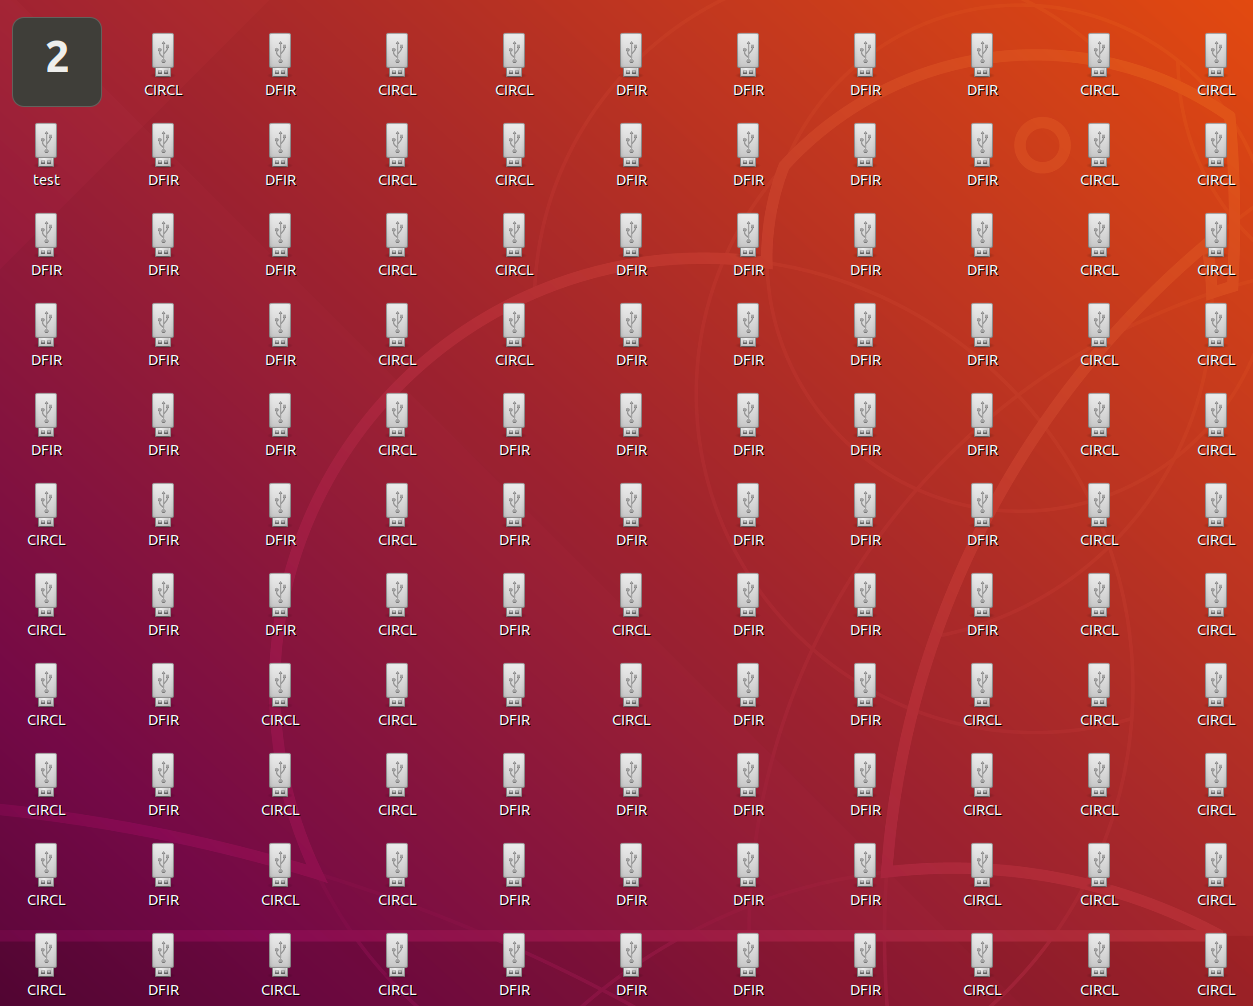
\includegraphics[scale=0.2]{images/ebr.png}
\end{frame}


\begin{frame}[fragile]
    \frametitle{6.3 Lost in Hyperspace: USB stick investigation}
  \begin{lstlisting}[basicstyle=\tiny]
$ fdisk -l /dev/sdb

     Device        Boot  Start    End Sectors  Size Id Type
     /dev/sdb1            2048 264191  262144  128M  5 Extended
     /dev/sdb5            4096  20479   16384    8M  7 HPFS/NTFS/exFAT
     /dev/sdb6           22528 120831   98304   48M  7 HPFS/NTFS/exFAT
     /dev/sdb7          122880 253951  131072   64M  7 HPFS/NTFS/exFAT
     /dev/sdb8           22528 120831   98304   48M  7 HPFS/NTFS/exFAT
     /dev/sdb9          122880 253951  131072   64M  7 HPFS/NTFS/exFAT
          .....
          .....
     /dev/sdb56          22528 120831   98304   48M  7 HPFS/NTFS/exFAT
     /dev/sdb57         122880 253951  131072   64M  7 HPFS/NTFS/exFAT
     /dev/sdb58          22528 120831   98304   48M  7 HPFS/NTFS/exFAT
     /dev/sdb59         122880 253951  131072   64M  7 HPFS/NTFS/exFAT
     /dev/sdb60          22528 120831   98304   48M  7 HPFS/NTFS/exFAT

$ mount
          .....
     /dev/sdb79 on /media/michael/DFIR25
     /dev/sdb82 on /media/michael/CIRCL28
     /dev/sdb86 on /media/michael/CIRCL33 
          .....
          .....
     /dev/sdb162 on /media/michael/CIRCL68
     /dev/sdb163 on /media/michael/DFIR73
     /dev/sdb166 on /media/michael/CIRCL64
  \end{lstlisting}
\end{frame}


\begin{frame}[fragile]
    \frametitle{6.3 Lost in Hyperspace: USB stick investigation}
    \begin{itemize}
	    \item[] Do further investigations:
  \begin{lstlisting}[basicstyle=\tiny]
$ df -ha

          .....
     /dev/sdb157           64M  2,5M   62M   4% /media/michael/DFIR72
     /dev/sdb158           48M  2,5M   46M   6% /media/michael/CIRCL63
     /dev/sdb159           64M  2,5M   62M   4% /media/michael/DFIR69
     /dev/sdb160           48M  2,5M   46M   6% /media/michael/CIRCL67
     /dev/sdb162           48M  2,5M   46M   6% /media/michael/CIRCL68
     /dev/sdb163           64M  2,5M   62M   4% /media/michael/DFIR73
          .....


$ mmls /dev/sdb                         --> Nothing... WTF?


  \end{lstlisting}
	    \item[] Any ideas how to proceed?
	    \item[] $\to$ Use hexeditor to read the partition table
    \end{itemize}
\end{frame}


\begin{frame}[fragile]
    \frametitle{6.3 Lost in Hyperspace: Solution step 1}
  \begin{lstlisting}[basicstyle=\tiny]
                           Extended Partition Container                          
------------------------------------------------------------------------------------
|EBR|000|     Logical     |                                                        |
------------------------------------------------------------------------------------
    --->                  ---------------------------
    --------------------> |EBR|000|     Logical     |
    Extended Partition    ---------------------------
                              --->                  ---------------------
                              --------------------> |EBR|000|  Logical  |
                              Extended Partition    ---------------------
                                                        --->



EBR_01:  001001b0: 0000 0000 0000 0000 0000 0000 0000 0029
         001001c0: 0708 0717 0a2c 0008 0000 0040 0000 0018
         001001d0: 012c 051f 4206 0048 0000 0088 0100 0000

         EBR_02:  00A001B0: 0000 0000 0000 0000 0000 0000 0000 002C
                  00A001C0: 0930 071F 4206 0008 0000 0080 0100 001F
                  00A001D0: 4306 0503 8228 00D0 0100 0008 0200 0000

                  EBR_03:  03B001B0: 0000 0000 0000 0000 0000 0000 0000 0006
                           03B001C0: 410B 0703 8228 0008 0000 0000 0200 0000
                           03B001D0: 0000 0000 0000 0000 0000 0000 0000 0000
  \end{lstlisting}
\end{frame}


\begin{frame}[fragile]
    \frametitle{6.3 Lost in Hyperspace: Solution step 2}
\begin{lstlisting}[basicstyle=\tiny]
                           Extended Partition Container                          
------------------------------------------------------------------------------------
|EBR|000|     Logical     |                                                        |
------------------------------------------------------------------------------------
    --->                  ---------------------------
    --------------------> |EBR|000|     Logical     |
    Extended Partition    ---------------------------
                              --->                  ---------------------
                              --------------------> |EBR|000|  Logical  |
                              Extended Partition    ---------------------
                                                        --->
                           <-----------------------------


EBR_01:  001001b0: 0000 0000 0000 0000 0000 0000 0000 0029
         001001c0: 0708 0717 0a2c 0008 0000 0040 0000 0018
         001001d0: 012c 051f 4206 0048 0000 0088 0100 0000

         EBR_02:  00A001B0: 0000 0000 0000 0000 0000 0000 0000 002C
                  00A001C0: 0930 071F 4206 0008 0000 0080 0100 001F
                  00A001D0: 4306 0503 8228 00D0 0100 0008 0200 0000

                  EBR_03:  03B001B0: 0000 0000 0000 0000 0000 0000 0000 0006
                           03B001C0: 410B 0703 8228 0008 0000 0000 0200 0000
                           03B001D0: 0000 0500 0000 0048 0000 0088 0100 0000
  \end{lstlisting}
\end{frame}




